% Created by tikzDevice version 0.9 on 2016-01-07 11:04:56
% !TEX encoding = UTF-8 Unicode
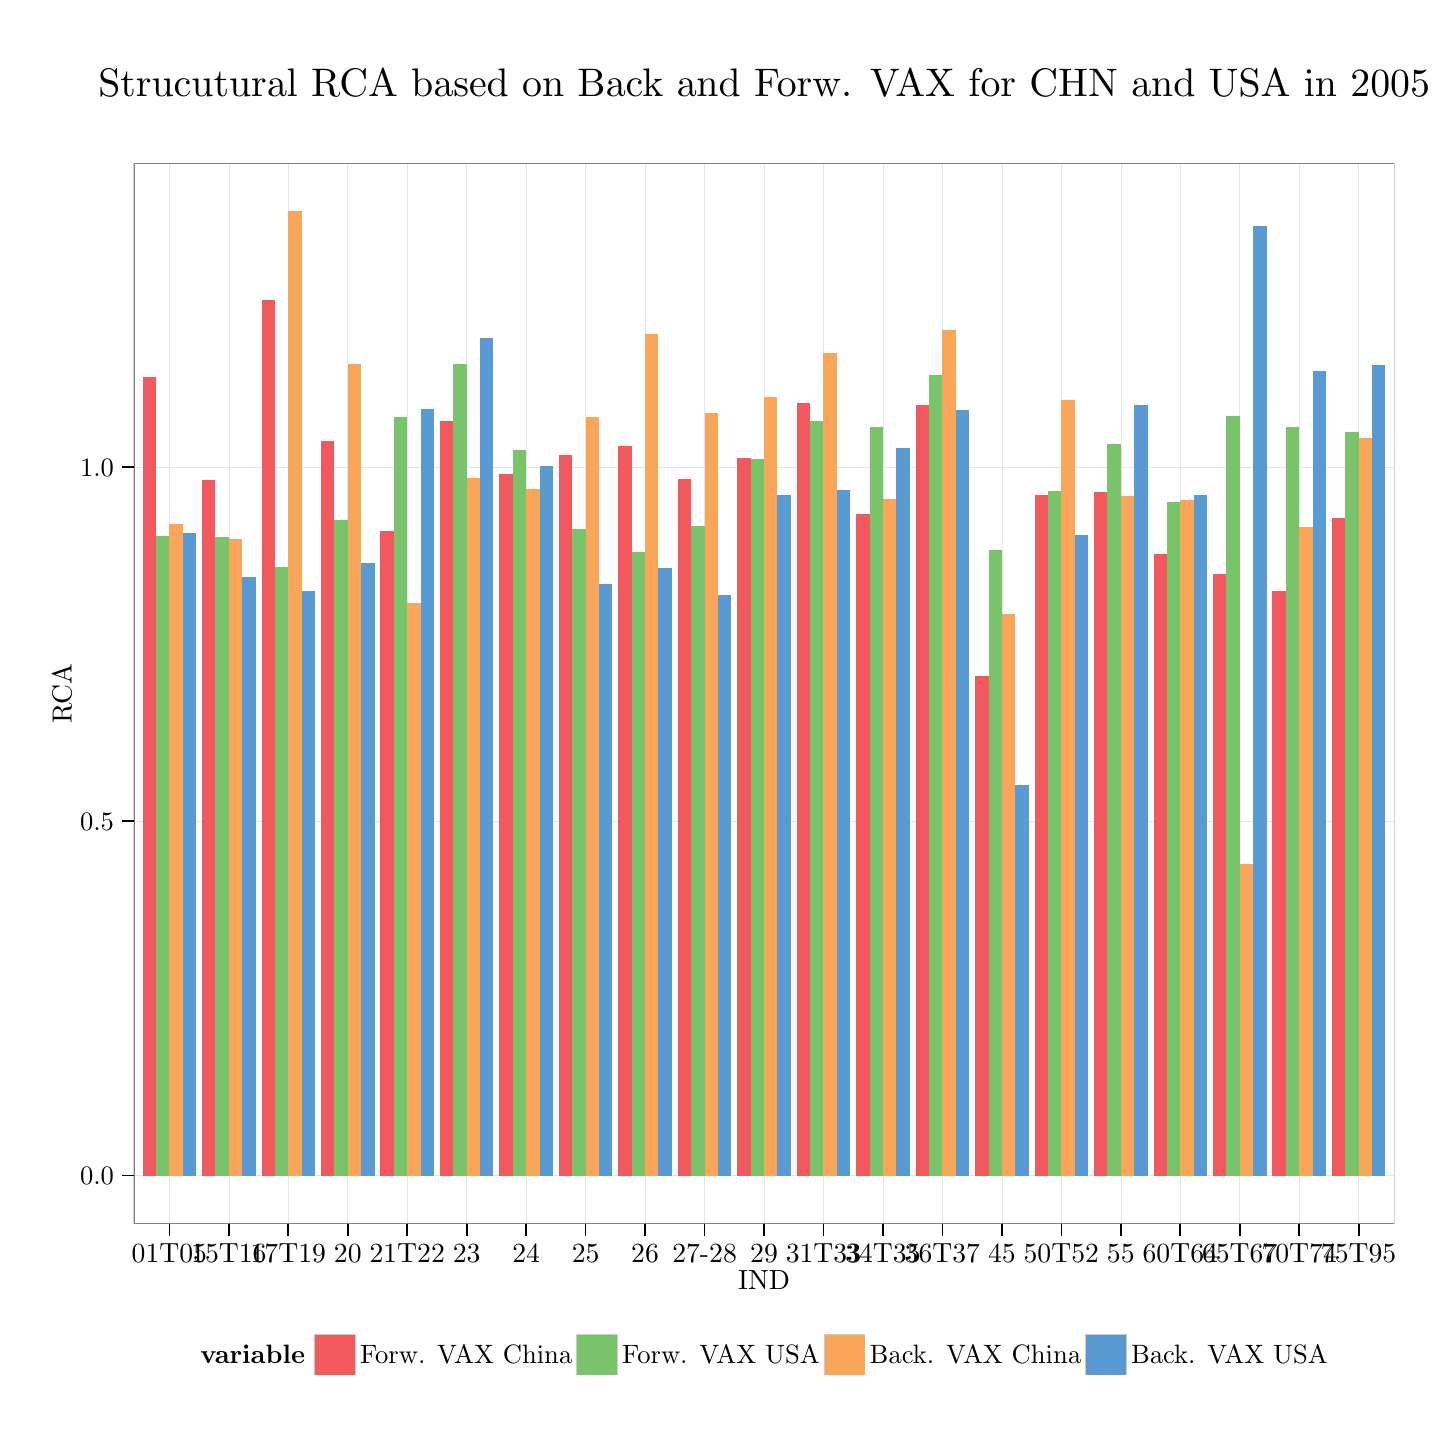
\begin{tikzpicture}[x=1pt,y=1pt]
\definecolor{fillColor}{RGB}{255,255,255}
\path[use as bounding box,fill=fillColor,fill opacity=0.00] (0,0) rectangle (505.89,505.89);
\begin{scope}
\path[clip] (  0.00,  0.00) rectangle (505.89,505.89);
\definecolor{drawColor}{RGB}{255,255,255}
\definecolor{fillColor}{RGB}{255,255,255}

\path[draw=drawColor,line width= 0.6pt,line join=round,line cap=round,fill=fillColor] (  0.00, -0.00) rectangle (505.89,505.89);
\end{scope}
\begin{scope}
\path[clip] ( 38.31, 73.66) rectangle (493.85,456.97);
\definecolor{fillColor}{RGB}{255,255,255}

\path[fill=fillColor] ( 38.31, 73.66) rectangle (493.85,456.97);
\definecolor{drawColor}{gray}{0.90}

\path[draw=drawColor,line width= 0.2pt,line join=round] ( 38.31, 91.08) --
	(493.85, 91.08);

\path[draw=drawColor,line width= 0.2pt,line join=round] ( 38.31,219.14) --
	(493.85,219.14);

\path[draw=drawColor,line width= 0.2pt,line join=round] ( 38.31,347.19) --
	(493.85,347.19);

\path[draw=drawColor,line width= 0.2pt,line join=round] ( 51.20, 73.66) --
	( 51.20,456.97);

\path[draw=drawColor,line width= 0.2pt,line join=round] ( 72.69, 73.66) --
	( 72.69,456.97);

\path[draw=drawColor,line width= 0.2pt,line join=round] ( 94.18, 73.66) --
	( 94.18,456.97);

\path[draw=drawColor,line width= 0.2pt,line join=round] (115.66, 73.66) --
	(115.66,456.97);

\path[draw=drawColor,line width= 0.2pt,line join=round] (137.15, 73.66) --
	(137.15,456.97);

\path[draw=drawColor,line width= 0.2pt,line join=round] (158.64, 73.66) --
	(158.64,456.97);

\path[draw=drawColor,line width= 0.2pt,line join=round] (180.13, 73.66) --
	(180.13,456.97);

\path[draw=drawColor,line width= 0.2pt,line join=round] (201.61, 73.66) --
	(201.61,456.97);

\path[draw=drawColor,line width= 0.2pt,line join=round] (223.10, 73.66) --
	(223.10,456.97);

\path[draw=drawColor,line width= 0.2pt,line join=round] (244.59, 73.66) --
	(244.59,456.97);

\path[draw=drawColor,line width= 0.2pt,line join=round] (266.08, 73.66) --
	(266.08,456.97);

\path[draw=drawColor,line width= 0.2pt,line join=round] (287.56, 73.66) --
	(287.56,456.97);

\path[draw=drawColor,line width= 0.2pt,line join=round] (309.05, 73.66) --
	(309.05,456.97);

\path[draw=drawColor,line width= 0.2pt,line join=round] (330.54, 73.66) --
	(330.54,456.97);

\path[draw=drawColor,line width= 0.2pt,line join=round] (352.03, 73.66) --
	(352.03,456.97);

\path[draw=drawColor,line width= 0.2pt,line join=round] (373.51, 73.66) --
	(373.51,456.97);

\path[draw=drawColor,line width= 0.2pt,line join=round] (395.00, 73.66) --
	(395.00,456.97);

\path[draw=drawColor,line width= 0.2pt,line join=round] (416.49, 73.66) --
	(416.49,456.97);

\path[draw=drawColor,line width= 0.2pt,line join=round] (437.98, 73.66) --
	(437.98,456.97);

\path[draw=drawColor,line width= 0.2pt,line join=round] (459.46, 73.66) --
	(459.46,456.97);

\path[draw=drawColor,line width= 0.2pt,line join=round] (480.95, 73.66) --
	(480.95,456.97);
\definecolor{fillColor}{RGB}{241,89,95}

\path[fill=fillColor] ( 41.53, 91.08) rectangle ( 46.37,379.75);
\definecolor{fillColor}{RGB}{121,195,106}

\path[fill=fillColor] ( 46.37, 91.08) rectangle ( 51.20,322.35);
\definecolor{fillColor}{RGB}{249,166,90}

\path[fill=fillColor] ( 51.20, 91.08) rectangle ( 56.04,326.46);
\definecolor{fillColor}{RGB}{89,154,211}

\path[fill=fillColor] ( 56.04, 91.08) rectangle ( 60.87,323.37);
\definecolor{fillColor}{RGB}{241,89,95}

\path[fill=fillColor] ( 63.02, 91.08) rectangle ( 67.85,342.54);
\definecolor{fillColor}{RGB}{121,195,106}

\path[fill=fillColor] ( 67.85, 91.08) rectangle ( 72.69,321.89);
\definecolor{fillColor}{RGB}{249,166,90}

\path[fill=fillColor] ( 72.69, 91.08) rectangle ( 77.52,321.08);
\definecolor{fillColor}{RGB}{89,154,211}

\path[fill=fillColor] ( 77.52, 91.08) rectangle ( 82.36,307.51);
\definecolor{fillColor}{RGB}{241,89,95}

\path[fill=fillColor] ( 84.51, 91.08) rectangle ( 89.34,407.41);
\definecolor{fillColor}{RGB}{121,195,106}

\path[fill=fillColor] ( 89.34, 91.08) rectangle ( 94.18,310.83);
\definecolor{fillColor}{RGB}{249,166,90}

\path[fill=fillColor] ( 94.18, 91.08) rectangle ( 99.01,439.54);
\definecolor{fillColor}{RGB}{89,154,211}

\path[fill=fillColor] ( 99.01, 91.08) rectangle (103.85,302.41);
\definecolor{fillColor}{RGB}{241,89,95}

\path[fill=fillColor] (105.99, 91.08) rectangle (110.83,356.47);
\definecolor{fillColor}{RGB}{121,195,106}

\path[fill=fillColor] (110.83, 91.08) rectangle (115.66,327.95);
\definecolor{fillColor}{RGB}{249,166,90}

\path[fill=fillColor] (115.66, 91.08) rectangle (120.50,384.52);
\definecolor{fillColor}{RGB}{89,154,211}

\path[fill=fillColor] (120.50, 91.08) rectangle (125.33,312.30);
\definecolor{fillColor}{RGB}{241,89,95}

\path[fill=fillColor] (127.48, 91.08) rectangle (132.32,323.85);
\definecolor{fillColor}{RGB}{121,195,106}

\path[fill=fillColor] (132.32, 91.08) rectangle (137.15,365.21);
\definecolor{fillColor}{RGB}{249,166,90}

\path[fill=fillColor] (137.15, 91.08) rectangle (141.99,298.11);
\definecolor{fillColor}{RGB}{89,154,211}

\path[fill=fillColor] (141.99, 91.08) rectangle (146.82,368.23);
\definecolor{fillColor}{RGB}{241,89,95}

\path[fill=fillColor] (148.97, 91.08) rectangle (153.80,363.69);
\definecolor{fillColor}{RGB}{121,195,106}

\path[fill=fillColor] (153.80, 91.08) rectangle (158.64,384.24);
\definecolor{fillColor}{RGB}{249,166,90}

\path[fill=fillColor] (158.64, 91.08) rectangle (163.47,343.16);
\definecolor{fillColor}{RGB}{89,154,211}

\path[fill=fillColor] (163.47, 91.08) rectangle (168.31,393.69);
\definecolor{fillColor}{RGB}{241,89,95}

\path[fill=fillColor] (170.46, 91.08) rectangle (175.29,344.62);
\definecolor{fillColor}{RGB}{121,195,106}

\path[fill=fillColor] (175.29, 91.08) rectangle (180.13,353.17);
\definecolor{fillColor}{RGB}{249,166,90}

\path[fill=fillColor] (180.13, 91.08) rectangle (184.96,339.14);
\definecolor{fillColor}{RGB}{89,154,211}

\path[fill=fillColor] (184.96, 91.08) rectangle (189.80,347.63);
\definecolor{fillColor}{RGB}{241,89,95}

\path[fill=fillColor] (191.95, 91.08) rectangle (196.78,351.39);
\definecolor{fillColor}{RGB}{121,195,106}

\path[fill=fillColor] (196.78, 91.08) rectangle (201.61,324.87);
\definecolor{fillColor}{RGB}{249,166,90}

\path[fill=fillColor] (201.61, 91.08) rectangle (206.45,365.15);
\definecolor{fillColor}{RGB}{89,154,211}

\path[fill=fillColor] (206.45, 91.08) rectangle (211.28,304.96);
\definecolor{fillColor}{RGB}{241,89,95}

\path[fill=fillColor] (213.43, 91.08) rectangle (218.27,354.86);
\definecolor{fillColor}{RGB}{121,195,106}

\path[fill=fillColor] (218.27, 91.08) rectangle (223.10,316.39);
\definecolor{fillColor}{RGB}{249,166,90}

\path[fill=fillColor] (223.10, 91.08) rectangle (227.94,395.28);
\definecolor{fillColor}{RGB}{89,154,211}

\path[fill=fillColor] (227.94, 91.08) rectangle (232.77,310.58);
\definecolor{fillColor}{RGB}{241,89,95}

\path[fill=fillColor] (234.92, 91.08) rectangle (239.75,342.63);
\definecolor{fillColor}{RGB}{121,195,106}

\path[fill=fillColor] (239.75, 91.08) rectangle (244.59,325.71);
\definecolor{fillColor}{RGB}{249,166,90}

\path[fill=fillColor] (244.59, 91.08) rectangle (249.42,366.70);
\definecolor{fillColor}{RGB}{89,154,211}

\path[fill=fillColor] (249.42, 91.08) rectangle (254.26,300.71);
\definecolor{fillColor}{RGB}{241,89,95}

\path[fill=fillColor] (256.41, 91.08) rectangle (261.24,350.41);
\definecolor{fillColor}{RGB}{121,195,106}

\path[fill=fillColor] (261.24, 91.08) rectangle (266.08,350.05);
\definecolor{fillColor}{RGB}{249,166,90}

\path[fill=fillColor] (266.08, 91.08) rectangle (270.91,372.33);
\definecolor{fillColor}{RGB}{89,154,211}

\path[fill=fillColor] (270.91, 91.08) rectangle (275.75,337.09);
\definecolor{fillColor}{RGB}{241,89,95}

\path[fill=fillColor] (277.90, 91.08) rectangle (282.73,370.16);
\definecolor{fillColor}{RGB}{121,195,106}

\path[fill=fillColor] (282.73, 91.08) rectangle (287.56,363.87);
\definecolor{fillColor}{RGB}{249,166,90}

\path[fill=fillColor] (287.56, 91.08) rectangle (292.40,388.26);
\definecolor{fillColor}{RGB}{89,154,211}

\path[fill=fillColor] (292.40, 91.08) rectangle (297.23,338.78);
\definecolor{fillColor}{RGB}{241,89,95}

\path[fill=fillColor] (299.38, 91.08) rectangle (304.22,330.11);
\definecolor{fillColor}{RGB}{121,195,106}

\path[fill=fillColor] (304.22, 91.08) rectangle (309.05,361.71);
\definecolor{fillColor}{RGB}{249,166,90}

\path[fill=fillColor] (309.05, 91.08) rectangle (313.89,335.44);
\definecolor{fillColor}{RGB}{89,154,211}

\path[fill=fillColor] (313.89, 91.08) rectangle (318.72,353.93);
\definecolor{fillColor}{RGB}{241,89,95}

\path[fill=fillColor] (320.87, 91.08) rectangle (325.70,369.42);
\definecolor{fillColor}{RGB}{121,195,106}

\path[fill=fillColor] (325.70, 91.08) rectangle (330.54,380.41);
\definecolor{fillColor}{RGB}{249,166,90}

\path[fill=fillColor] (330.54, 91.08) rectangle (335.37,396.69);
\definecolor{fillColor}{RGB}{89,154,211}

\path[fill=fillColor] (335.37, 91.08) rectangle (340.21,367.78);
\definecolor{fillColor}{RGB}{241,89,95}

\path[fill=fillColor] (342.36, 91.08) rectangle (347.19,271.63);
\definecolor{fillColor}{RGB}{121,195,106}

\path[fill=fillColor] (347.19, 91.08) rectangle (352.03,316.97);
\definecolor{fillColor}{RGB}{249,166,90}

\path[fill=fillColor] (352.03, 91.08) rectangle (356.86,293.90);
\definecolor{fillColor}{RGB}{89,154,211}

\path[fill=fillColor] (356.86, 91.08) rectangle (361.70,232.27);
\definecolor{fillColor}{RGB}{241,89,95}

\path[fill=fillColor] (363.85, 91.08) rectangle (368.68,336.96);
\definecolor{fillColor}{RGB}{121,195,106}

\path[fill=fillColor] (368.68, 91.08) rectangle (373.51,338.55);
\definecolor{fillColor}{RGB}{249,166,90}

\path[fill=fillColor] (373.51, 91.08) rectangle (378.35,371.28);
\definecolor{fillColor}{RGB}{89,154,211}

\path[fill=fillColor] (378.35, 91.08) rectangle (383.18,322.48);
\definecolor{fillColor}{RGB}{241,89,95}

\path[fill=fillColor] (385.33, 91.08) rectangle (390.17,338.03);
\definecolor{fillColor}{RGB}{121,195,106}

\path[fill=fillColor] (390.17, 91.08) rectangle (395.00,355.53);
\definecolor{fillColor}{RGB}{249,166,90}

\path[fill=fillColor] (395.00, 91.08) rectangle (399.84,336.83);
\definecolor{fillColor}{RGB}{89,154,211}

\path[fill=fillColor] (399.84, 91.08) rectangle (404.67,369.69);
\definecolor{fillColor}{RGB}{241,89,95}

\path[fill=fillColor] (406.82, 91.08) rectangle (411.66,315.57);
\definecolor{fillColor}{RGB}{121,195,106}

\path[fill=fillColor] (411.66, 91.08) rectangle (416.49,334.62);
\definecolor{fillColor}{RGB}{249,166,90}

\path[fill=fillColor] (416.49, 91.08) rectangle (421.32,335.05);
\definecolor{fillColor}{RGB}{89,154,211}

\path[fill=fillColor] (421.32, 91.08) rectangle (426.16,336.95);
\definecolor{fillColor}{RGB}{241,89,95}

\path[fill=fillColor] (428.31, 91.08) rectangle (433.14,308.41);
\definecolor{fillColor}{RGB}{121,195,106}

\path[fill=fillColor] (433.14, 91.08) rectangle (437.98,365.40);
\definecolor{fillColor}{RGB}{249,166,90}

\path[fill=fillColor] (437.98, 91.08) rectangle (442.81,203.77);
\definecolor{fillColor}{RGB}{89,154,211}

\path[fill=fillColor] (442.81, 91.08) rectangle (447.65,434.20);
\definecolor{fillColor}{RGB}{241,89,95}

\path[fill=fillColor] (449.80, 91.08) rectangle (454.63,302.16);
\definecolor{fillColor}{RGB}{121,195,106}

\path[fill=fillColor] (454.63, 91.08) rectangle (459.46,361.56);
\definecolor{fillColor}{RGB}{249,166,90}

\path[fill=fillColor] (459.46, 91.08) rectangle (464.30,325.60);
\definecolor{fillColor}{RGB}{89,154,211}

\path[fill=fillColor] (464.30, 91.08) rectangle (469.13,381.84);
\definecolor{fillColor}{RGB}{241,89,95}

\path[fill=fillColor] (471.28, 91.08) rectangle (476.12,328.68);
\definecolor{fillColor}{RGB}{121,195,106}

\path[fill=fillColor] (476.12, 91.08) rectangle (480.95,359.74);
\definecolor{fillColor}{RGB}{249,166,90}

\path[fill=fillColor] (480.95, 91.08) rectangle (485.79,357.52);
\definecolor{fillColor}{RGB}{89,154,211}

\path[fill=fillColor] (485.79, 91.08) rectangle (490.62,383.89);
\definecolor{drawColor}{gray}{0.50}

\path[draw=drawColor,line width= 0.6pt,line join=round,line cap=round] ( 38.31, 73.66) rectangle (493.85,456.97);
\end{scope}
\begin{scope}
\path[clip] (  0.00,  0.00) rectangle (505.89,505.89);
\definecolor{drawColor}{RGB}{0,0,0}

\node[text=drawColor,anchor=base east,inner sep=0pt, outer sep=0pt, scale=  0.96] at ( 31.20, 87.78) {0.0};

\node[text=drawColor,anchor=base east,inner sep=0pt, outer sep=0pt, scale=  0.96] at ( 31.20,215.83) {0.5};

\node[text=drawColor,anchor=base east,inner sep=0pt, outer sep=0pt, scale=  0.96] at ( 31.20,343.88) {1.0};
\end{scope}
\begin{scope}
\path[clip] (  0.00,  0.00) rectangle (505.89,505.89);
\definecolor{drawColor}{RGB}{0,0,0}

\path[draw=drawColor,line width= 0.6pt,line join=round] ( 34.04, 91.08) --
	( 38.31, 91.08);

\path[draw=drawColor,line width= 0.6pt,line join=round] ( 34.04,219.14) --
	( 38.31,219.14);

\path[draw=drawColor,line width= 0.6pt,line join=round] ( 34.04,347.19) --
	( 38.31,347.19);
\end{scope}
\begin{scope}
\path[clip] (  0.00,  0.00) rectangle (505.89,505.89);
\definecolor{drawColor}{RGB}{0,0,0}

\path[draw=drawColor,line width= 0.6pt,line join=round] ( 51.20, 69.39) --
	( 51.20, 73.66);

\path[draw=drawColor,line width= 0.6pt,line join=round] ( 72.69, 69.39) --
	( 72.69, 73.66);

\path[draw=drawColor,line width= 0.6pt,line join=round] ( 94.18, 69.39) --
	( 94.18, 73.66);

\path[draw=drawColor,line width= 0.6pt,line join=round] (115.66, 69.39) --
	(115.66, 73.66);

\path[draw=drawColor,line width= 0.6pt,line join=round] (137.15, 69.39) --
	(137.15, 73.66);

\path[draw=drawColor,line width= 0.6pt,line join=round] (158.64, 69.39) --
	(158.64, 73.66);

\path[draw=drawColor,line width= 0.6pt,line join=round] (180.13, 69.39) --
	(180.13, 73.66);

\path[draw=drawColor,line width= 0.6pt,line join=round] (201.61, 69.39) --
	(201.61, 73.66);

\path[draw=drawColor,line width= 0.6pt,line join=round] (223.10, 69.39) --
	(223.10, 73.66);

\path[draw=drawColor,line width= 0.6pt,line join=round] (244.59, 69.39) --
	(244.59, 73.66);

\path[draw=drawColor,line width= 0.6pt,line join=round] (266.08, 69.39) --
	(266.08, 73.66);

\path[draw=drawColor,line width= 0.6pt,line join=round] (287.56, 69.39) --
	(287.56, 73.66);

\path[draw=drawColor,line width= 0.6pt,line join=round] (309.05, 69.39) --
	(309.05, 73.66);

\path[draw=drawColor,line width= 0.6pt,line join=round] (330.54, 69.39) --
	(330.54, 73.66);

\path[draw=drawColor,line width= 0.6pt,line join=round] (352.03, 69.39) --
	(352.03, 73.66);

\path[draw=drawColor,line width= 0.6pt,line join=round] (373.51, 69.39) --
	(373.51, 73.66);

\path[draw=drawColor,line width= 0.6pt,line join=round] (395.00, 69.39) --
	(395.00, 73.66);

\path[draw=drawColor,line width= 0.6pt,line join=round] (416.49, 69.39) --
	(416.49, 73.66);

\path[draw=drawColor,line width= 0.6pt,line join=round] (437.98, 69.39) --
	(437.98, 73.66);

\path[draw=drawColor,line width= 0.6pt,line join=round] (459.46, 69.39) --
	(459.46, 73.66);

\path[draw=drawColor,line width= 0.6pt,line join=round] (480.95, 69.39) --
	(480.95, 73.66);
\end{scope}
\begin{scope}
\path[clip] (  0.00,  0.00) rectangle (505.89,505.89);
\definecolor{drawColor}{RGB}{0,0,0}

\node[text=drawColor,anchor=base,inner sep=0pt, outer sep=0pt, scale=  1.00] at ( 51.20, 59.66) {01T05};

\node[text=drawColor,anchor=base,inner sep=0pt, outer sep=0pt, scale=  1.00] at ( 72.69, 59.66) {15T16};

\node[text=drawColor,anchor=base,inner sep=0pt, outer sep=0pt, scale=  1.00] at ( 94.18, 59.66) {17T19};

\node[text=drawColor,anchor=base,inner sep=0pt, outer sep=0pt, scale=  1.00] at (115.66, 59.66) {20};

\node[text=drawColor,anchor=base,inner sep=0pt, outer sep=0pt, scale=  1.00] at (137.15, 59.66) {21T22};

\node[text=drawColor,anchor=base,inner sep=0pt, outer sep=0pt, scale=  1.00] at (158.64, 59.66) {23};

\node[text=drawColor,anchor=base,inner sep=0pt, outer sep=0pt, scale=  1.00] at (180.13, 59.66) {24};

\node[text=drawColor,anchor=base,inner sep=0pt, outer sep=0pt, scale=  1.00] at (201.61, 59.66) {25};

\node[text=drawColor,anchor=base,inner sep=0pt, outer sep=0pt, scale=  1.00] at (223.10, 59.66) {26};

\node[text=drawColor,anchor=base,inner sep=0pt, outer sep=0pt, scale=  1.00] at (244.59, 59.66) {27-28};

\node[text=drawColor,anchor=base,inner sep=0pt, outer sep=0pt, scale=  1.00] at (266.08, 59.66) {29};

\node[text=drawColor,anchor=base,inner sep=0pt, outer sep=0pt, scale=  1.00] at (287.56, 59.66) {31T33};

\node[text=drawColor,anchor=base,inner sep=0pt, outer sep=0pt, scale=  1.00] at (309.05, 59.66) {34T35};

\node[text=drawColor,anchor=base,inner sep=0pt, outer sep=0pt, scale=  1.00] at (330.54, 59.66) {36T37};

\node[text=drawColor,anchor=base,inner sep=0pt, outer sep=0pt, scale=  1.00] at (352.03, 59.66) {45};

\node[text=drawColor,anchor=base,inner sep=0pt, outer sep=0pt, scale=  1.00] at (373.51, 59.66) {50T52};

\node[text=drawColor,anchor=base,inner sep=0pt, outer sep=0pt, scale=  1.00] at (395.00, 59.66) {55};

\node[text=drawColor,anchor=base,inner sep=0pt, outer sep=0pt, scale=  1.00] at (416.49, 59.66) {60T64};

\node[text=drawColor,anchor=base,inner sep=0pt, outer sep=0pt, scale=  1.00] at (437.98, 59.66) {65T67};

\node[text=drawColor,anchor=base,inner sep=0pt, outer sep=0pt, scale=  1.00] at (459.46, 59.66) {70T74};

\node[text=drawColor,anchor=base,inner sep=0pt, outer sep=0pt, scale=  1.00] at (480.95, 59.66) {75T95};
\end{scope}
\begin{scope}
\path[clip] (  0.00,  0.00) rectangle (505.89,505.89);
\definecolor{drawColor}{RGB}{0,0,0}

\node[text=drawColor,anchor=base,inner sep=0pt, outer sep=0pt, scale=  1.00] at (266.08, 49.76) {IND};
\end{scope}
\begin{scope}
\path[clip] (  0.00,  0.00) rectangle (505.89,505.89);
\definecolor{drawColor}{RGB}{0,0,0}

\node[text=drawColor,rotate= 90.00,anchor=base,inner sep=0pt, outer sep=0pt, scale=  1.00] at ( 15.92,265.31) {RCA};
\end{scope}
\begin{scope}
\path[clip] (  0.00,  0.00) rectangle (505.89,505.89);
\definecolor{fillColor}{RGB}{255,255,255}

\path[fill=fillColor] ( 58.14, 14.89) rectangle (474.01, 37.88);
\end{scope}
\begin{scope}
\path[clip] (  0.00,  0.00) rectangle (505.89,505.89);
\definecolor{drawColor}{RGB}{0,0,0}

\node[text=drawColor,anchor=base west,inner sep=0pt, outer sep=0pt, scale=  0.96] at ( 62.41, 23.07) {\bfseries variable};
\end{scope}
\begin{scope}
\path[clip] (  0.00,  0.00) rectangle (505.89,505.89);
\definecolor{drawColor}{gray}{0.80}
\definecolor{fillColor}{RGB}{255,255,255}

\path[draw=drawColor,line width= 0.6pt,line join=round,line cap=round,fill=fillColor] (103.83, 19.16) rectangle (118.29, 33.61);
\end{scope}
\begin{scope}
\path[clip] (  0.00,  0.00) rectangle (505.89,505.89);
\definecolor{fillColor}{RGB}{241,89,95}

\path[fill=fillColor] (103.83, 19.16) rectangle (118.29, 33.61);

\path[] (103.83, 19.16) --
	(118.29, 33.61);
\end{scope}
\begin{scope}
\path[clip] (  0.00,  0.00) rectangle (505.89,505.89);
\definecolor{drawColor}{gray}{0.80}
\definecolor{fillColor}{RGB}{255,255,255}

\path[draw=drawColor,line width= 0.6pt,line join=round,line cap=round,fill=fillColor] (198.58, 19.16) rectangle (213.03, 33.61);
\end{scope}
\begin{scope}
\path[clip] (  0.00,  0.00) rectangle (505.89,505.89);
\definecolor{fillColor}{RGB}{121,195,106}

\path[fill=fillColor] (198.58, 19.16) rectangle (213.03, 33.61);

\path[] (198.58, 19.16) --
	(213.03, 33.61);
\end{scope}
\begin{scope}
\path[clip] (  0.00,  0.00) rectangle (505.89,505.89);
\definecolor{drawColor}{gray}{0.80}
\definecolor{fillColor}{RGB}{255,255,255}

\path[draw=drawColor,line width= 0.6pt,line join=round,line cap=round,fill=fillColor] (287.99, 19.16) rectangle (302.44, 33.61);
\end{scope}
\begin{scope}
\path[clip] (  0.00,  0.00) rectangle (505.89,505.89);
\definecolor{fillColor}{RGB}{249,166,90}

\path[fill=fillColor] (287.99, 19.16) rectangle (302.44, 33.61);

\path[] (287.99, 19.16) --
	(302.44, 33.61);
\end{scope}
\begin{scope}
\path[clip] (  0.00,  0.00) rectangle (505.89,505.89);
\definecolor{drawColor}{gray}{0.80}
\definecolor{fillColor}{RGB}{255,255,255}

\path[draw=drawColor,line width= 0.6pt,line join=round,line cap=round,fill=fillColor] (382.44, 19.16) rectangle (396.89, 33.61);
\end{scope}
\begin{scope}
\path[clip] (  0.00,  0.00) rectangle (505.89,505.89);
\definecolor{fillColor}{RGB}{89,154,211}

\path[fill=fillColor] (382.44, 19.16) rectangle (396.89, 33.61);

\path[] (382.44, 19.16) --
	(396.89, 33.61);
\end{scope}
\begin{scope}
\path[clip] (  0.00,  0.00) rectangle (505.89,505.89);
\definecolor{drawColor}{RGB}{0,0,0}

\node[text=drawColor,anchor=base west,inner sep=0pt, outer sep=0pt, scale=  0.96] at (120.09, 23.08) {Forw. VAX China};
\end{scope}
\begin{scope}
\path[clip] (  0.00,  0.00) rectangle (505.89,505.89);
\definecolor{drawColor}{RGB}{0,0,0}

\node[text=drawColor,anchor=base west,inner sep=0pt, outer sep=0pt, scale=  0.96] at (214.84, 23.08) {Forw. VAX USA};
\end{scope}
\begin{scope}
\path[clip] (  0.00,  0.00) rectangle (505.89,505.89);
\definecolor{drawColor}{RGB}{0,0,0}

\node[text=drawColor,anchor=base west,inner sep=0pt, outer sep=0pt, scale=  0.96] at (304.25, 23.08) {Back. VAX China};
\end{scope}
\begin{scope}
\path[clip] (  0.00,  0.00) rectangle (505.89,505.89);
\definecolor{drawColor}{RGB}{0,0,0}

\node[text=drawColor,anchor=base west,inner sep=0pt, outer sep=0pt, scale=  0.96] at (398.70, 23.08) {Back. VAX USA};
\end{scope}
\begin{scope}
\path[clip] (  0.00,  0.00) rectangle (505.89,505.89);
\definecolor{drawColor}{RGB}{0,0,0}

\node[text=drawColor,anchor=base west,inner sep=0pt, outer sep=0pt, scale=  1.44] at ( 25.52,480.92) {Strucutural RCA based on  Back and Forw. VAX for CHN and USA in 2005};
\end{scope}
\end{tikzpicture}
